Für die Bestimmung des Templates des korrelierten Untergrunds wird das Template des Signals von der Verteilung der invarianten Masse aus der Monte Carlo Simulation abgezogen, die im gleichen $p_\text{T}$-Intervall liegt wie das Template des Signals.
\begin{figure}[tp]
\centering
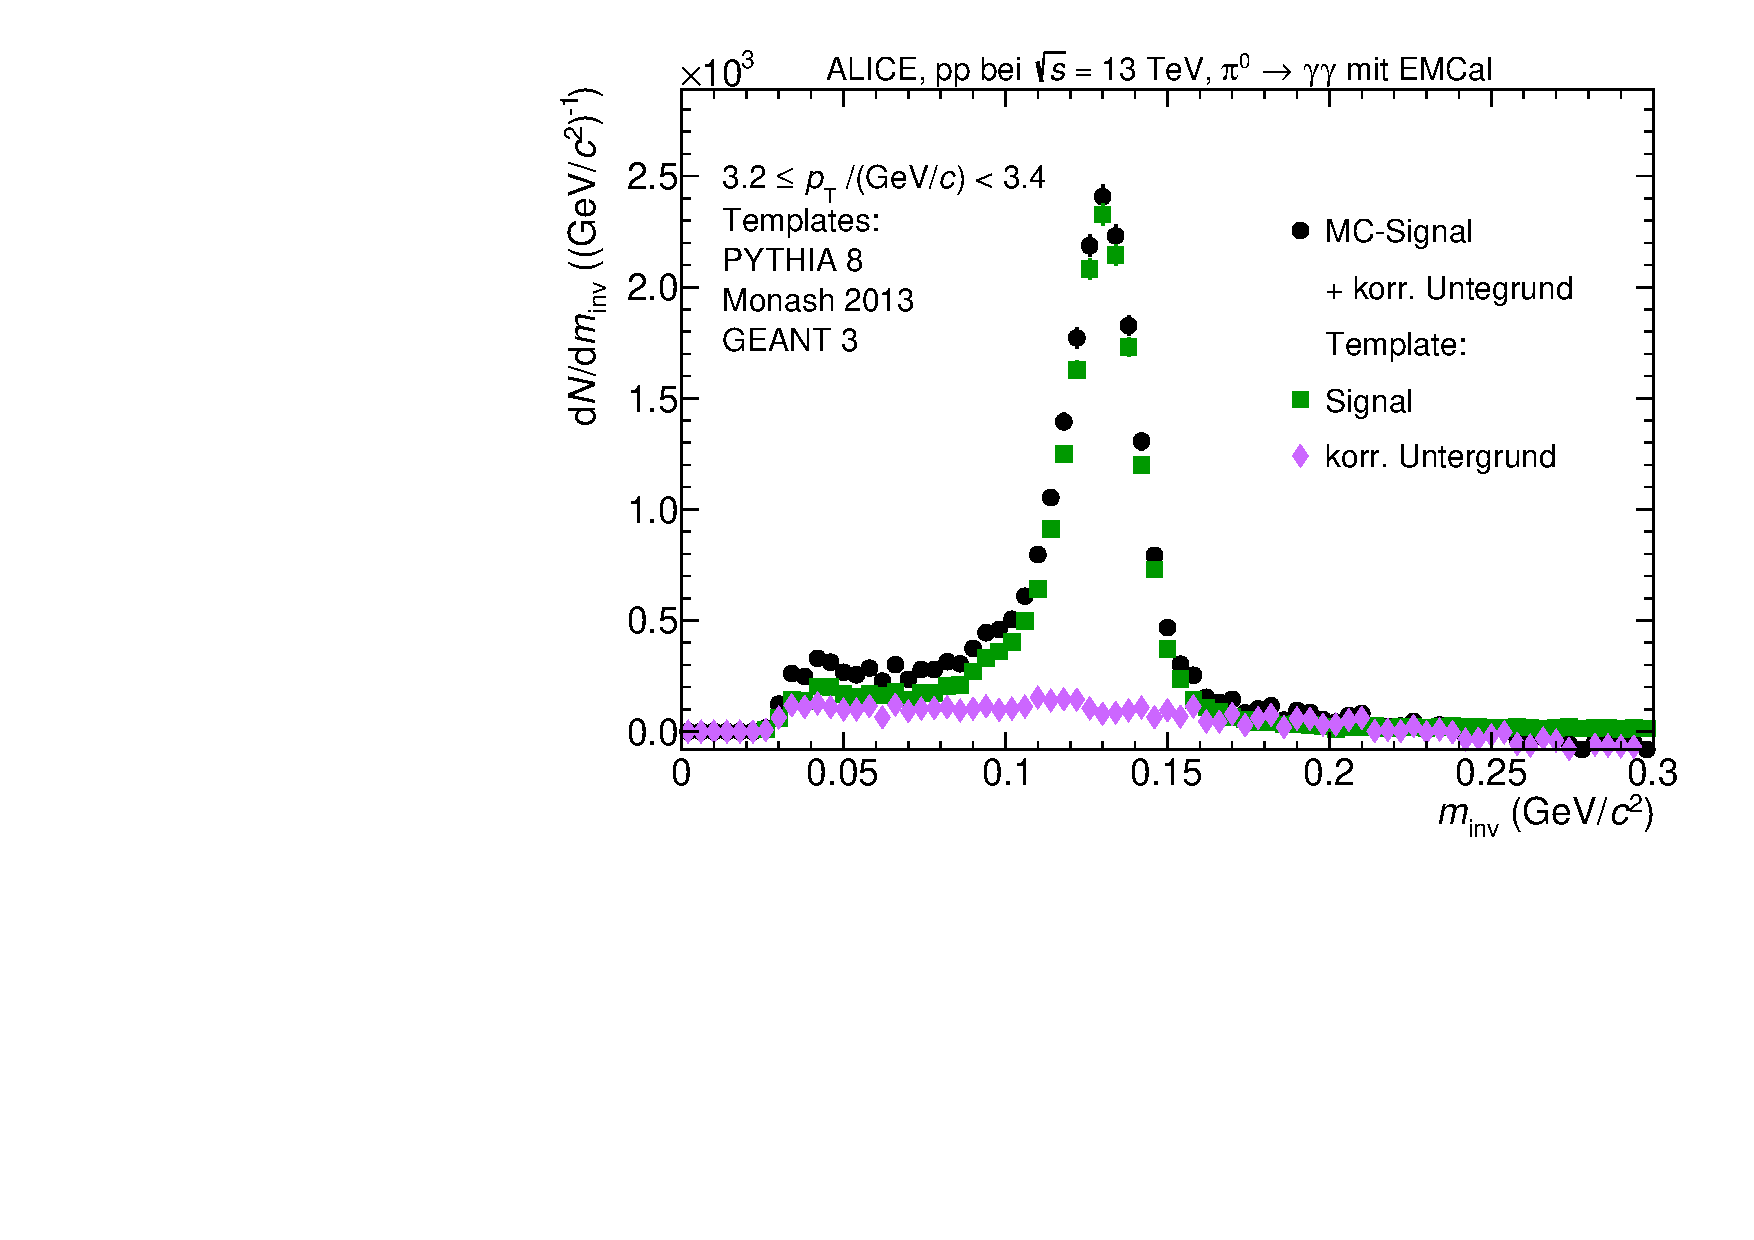
\includegraphics[width=.75\linewidth]{EntstehungUntergrund10_Data_2016.pdf}
\caption{Template des korrelierten Untergrunds in pink entstanden durch den Abzug des Templates des Signals (grün) von der Verteilung der invarianten Masse aus einer Monte Carlo Simulation (schwarz).}
\label{fig:BkgTemp}
\end{figure}
\newline
Abbildung \ref{fig:BkgTemp} zeigt die Anzahl \textit{Clusterpaare}, die aus dem Zerfall eines einzelnen $\pi^{0}$ stammen, als Funktion von $m_\text{inv}$ in schwarz.
In pink wird das Template des korrelierten Untergrunds dargestellt und in grün das Template des Signals.
Alle drei Verteilungen stammen aus dem $p_\text{T}$-Intervall $(3\,2 - 3\,4) (\text{GeV/}c)$.
Hierbei wird deutlich, dass in der Monte Carlo Simulation der korrelierte Untergrund im Bereich von $m_\text{inv} = 0,05 \text{ GeV/}c^{2}$ in der Größenordnung des Signals liegt.
In der Standardmethode wurde zuvor gezeigt, dass in diesem $m_\text{inv}$-Bereich der korrelierte Untergrund dominiert.
\newline
Für die Anpassung der Templates an die Daten wird, relativ zu den Werten der Einträge in den Templates, eine geringe statistische Unsicherheit der beiden Templates benötigt.
Um die Unsicherheit zu verkleinern wird in dieser Arbeit der korrelierte Untergrund aus einem größeren $p_\text{T}$-Intervallen verwendet, als die in dieser Analyse gewählten $p_\text{T}$-Intervalle.
Dieses Template wird im folgenden als kombiniertes Template des korrelierten Untergrunds bezeichnet, da das vergrößerte $p_\text{T}$-Intervall mehrere zuvor gewählten $p_\text{T}$-Intervalle kombiniert.
Dabei wird angenommen, dass sich nicht die Form, sondern nur die Anzahl der Einträge in den $p_\text{T}$-Intervallen unterscheidet.  
Für das kombinierte Template des korrelierten Untergrunds wird $p_\text{T} \geq 1\,8\text{ GeV}/c$ bis $p_\text{T} < 3\,2\text{ GeV}/c$ benutzt, da in diesem Bereich die statistische Unsicherheit am geringsten ist.
Um diese Methode zur Bestimmung des Template des korrelierten Untergrunds anwenden zu können, wird die Annahme getroffen, dass sich die Form des Template des korrelierten Untergrunds nicht ändert.
Lediglich die Anzahl der Einträge in den Templates des korrelierten Untergrunds variiert.
\begin{figure}[t!]
\centering
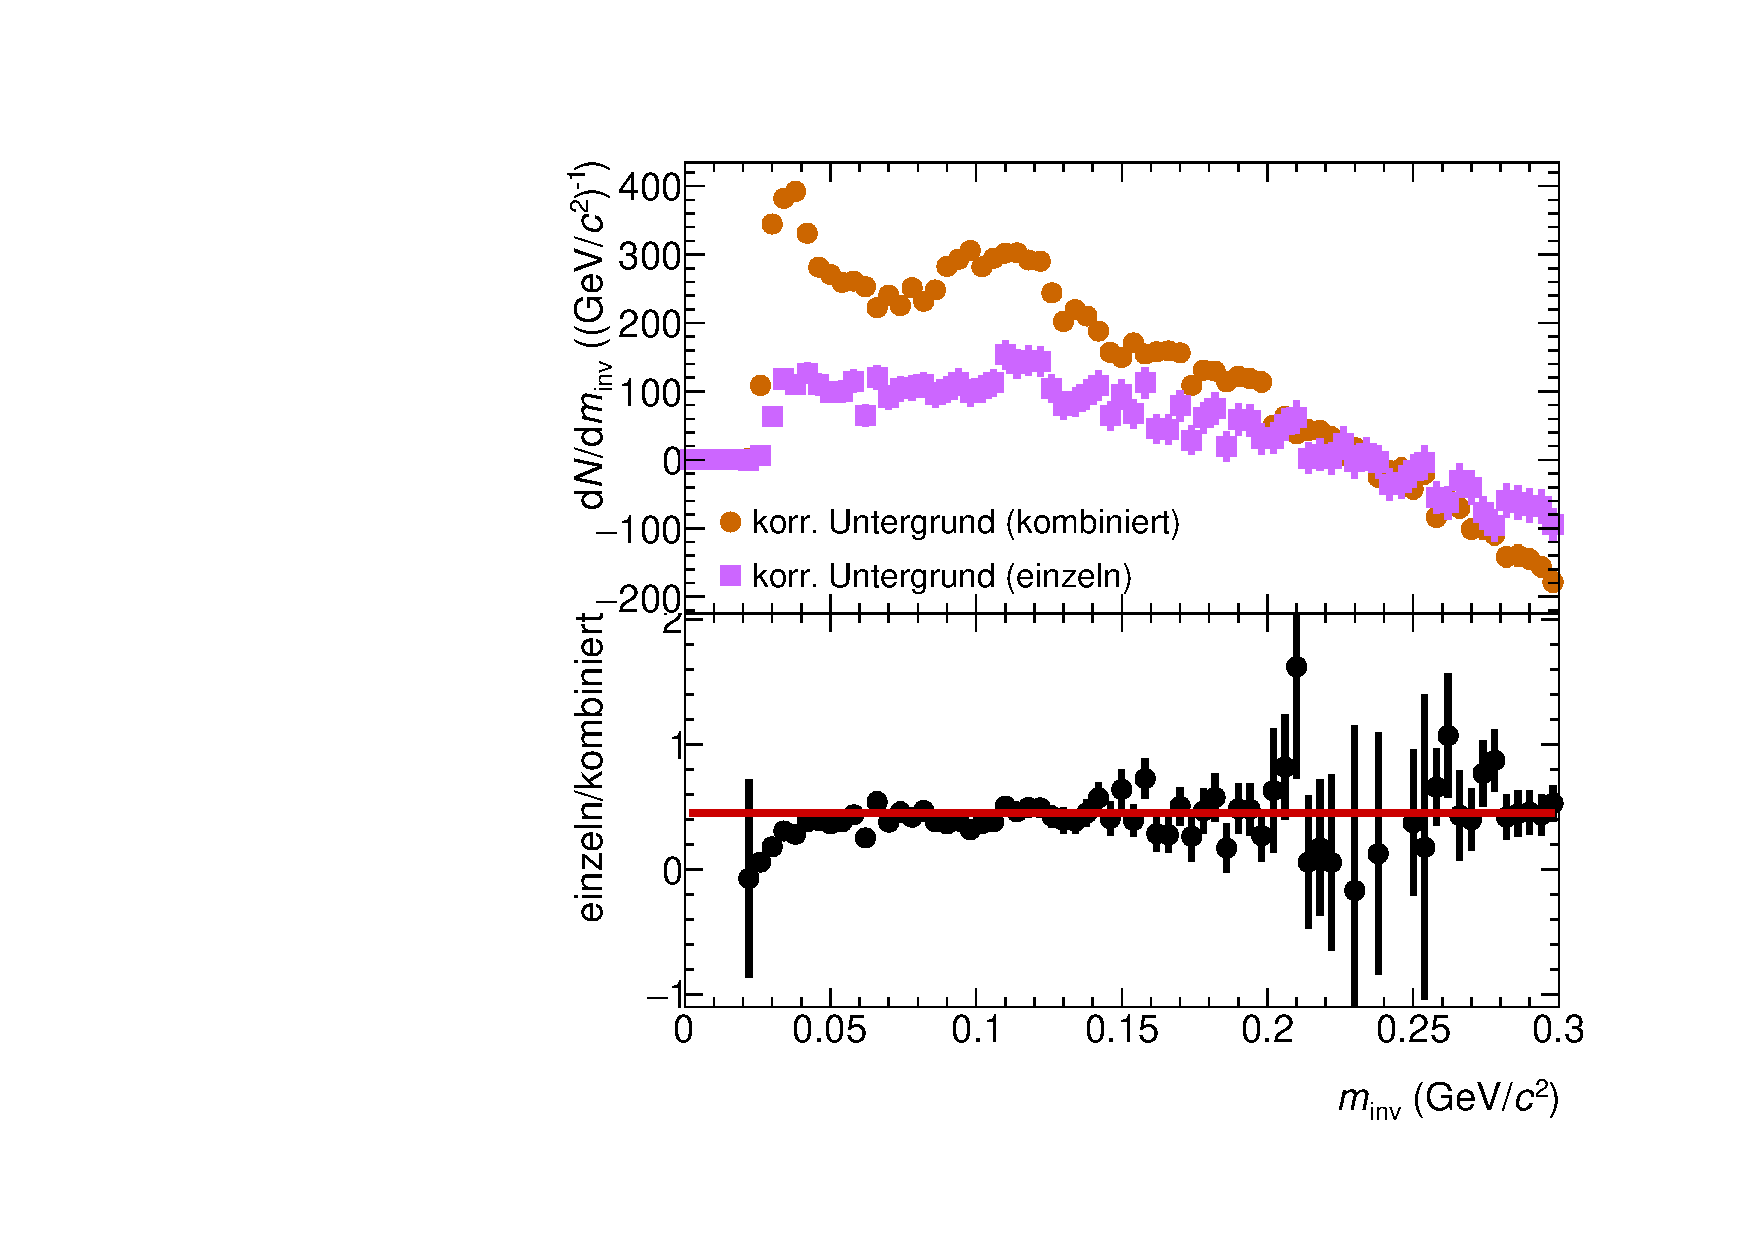
\includegraphics[width=.7\linewidth]{BackgroundWithRatio10_Data_2016.pdf}
\caption{\textbf{Oben:} Template des korrelierten Untergrunds aus einem einzelnen $p_\text{T}$-Intervall in pink und aus mehreren $p_\text{T}$-Intervallen kombiniert in orange.
\textbf{Unten:} Verhältnis der beiden Verteilungen in schwarz, sowie Parametrisierung einer Konstante an das Verhältnis in rot.}
\label{fig:BkgTempRatio}
\end{figure}
\newline
Abbildung \ref{fig:BkgTempRatio} (oben) zeigt in orange das kombiniertes Template des korrelierten Untergrunds und in pink das Template des korrelierten Untergrunds für das $p_\text{T}$-Intervall $(3\,2 - 3\,4) (\text{GeV/}c)$.
Um zu zeigen, dass die Annahme ihre Richtigkeit hat wird in Abbildung \ref{fig:BkgTempRatio} (unten) das Verhältnis aus einzelnen Templates des korrelierten Untergrunds zu dem Kombinierten dargestellt.
Die grüne Linie im unteren Teil der Abbildung basiert auf einer konstanten Parametrisierung des Verhältnisses.
Die getroffene Annahme wird bestätigt, da die konstante Parametrisierung und das Verhältnis gut miteinander übereinstimmen.
Die große Unsicherheit im Verhältnis um $m_\text{inv} = 0,225\text{ GeV}/c^{2}$ entsteht, da beide Templates an dieser Stelle eine Anzahl an Einträgen im Bereich nahe um die Null besitzen.
Teilt man zwei kleine Zahlen durch einander, so ändert sich der Quotientenwert stark, wenn man nur eine der beiden kleinen Zahlen leicht ändert.
Die Unsicherheit der Einträge der Templates repräsentieren eine mögliche Variation der Einträge.
Diese Unsicherheit im Falle des einzelnen Templates des korrelierten Untergrunds besitzt einen großen absoluten Wert verglichen mit den Werten der Einträge um $m_\text{inv} = 0,225\text{ GeV}/c^{2}$.
Dadurch wird auch die Unsicherheit auf den Quotientenwert deutlich größer, als in den anderen $m_\text{inv}$ Bereichen.
\newline
In Abschnitt \ref{s3s2} wurde bereits angesprochen, dass die Anforderung an den Öffnungswinkel von $p_\text{T}$ abhängt.
Um das kombinierte Template des korrelieren Untergrunds daran anzupassen wird eine für diesen Zweck angepasste Monte Carlo Simulation betrachtet.
In der Simulation werden $\pi^{0}$ mit zufälliger Energie simuliert, die in zwei Photonen zerfallen.
Die Photonen müssen dann auf einen Raumwinkel auftreten um als detektiert zu gelten, der der Abdeckung des EMCals entspricht.
Die Photonen werden hierbei nicht durch \textit{Cluster} repräsentiert.
Dadurch wird verhindert, dass mehrere Teilchen zu einem \textit{Cluster} zusammengefasst werden können.
Die Photonen werden paarweise kombiniert, wie bei der \textit{Clusterkombination}.
Dabei wird einmal die Anforderung an den Öffnungswinkel gestellt wie sie in der Analyse vorliegt und einmal wird keine Anforderung an den Öffnungswinkel gestellt.
In beiden Fällen werden so viele $\pi^{0}$ erzeugt, dass am Ende die gleiche Anzahl an Photonenpaaren kombiniert wurde.
Daraus entstehen zwei Verteilungen, die die Anzahl kombinierter Photonenpaare als Funktion von $m_\text{inv}$ und $p_\text{T}$ darstellen, einmal für den Fall, dass es keine Anforderung an den Öffnungswinkel gibt und einmal mit der Anforderung an den Öffnungswinkel.
Da beide Teilsimulationen die gleiche Anzahl an kombinierten Photonenpaaren haben, kann aus dem Verhältnis der Verteilung mit Anforderung an den Öffnungswinkel zur Verteilung ohne Anforderung an den Öffnungswinkel, bestimmt werden, wie wahrscheinlich es ist einen Photonenkombination bei einem bestimmen $m_\text{inv}$ und $p_\text{T}$ zu messen.
Mit Hilfe dieser Wahrscheinlichkeitsverteilung werden die Templates des korrelierten Untergrunds, die das kombinierte Template des korrelierten Untergrunds bilden, an die unterschiedlichen $p_\text{T}$-Intervalle skaliert.
Dadurch konnten größere Abweichungen für kleinere invariante Massen vermieden werden.
\newline
In Abschnitt \ref{s4s2} wird für die Bestimmung der systematischen Unsicherheit die Wahl des Templates des korrelierten Untergrunds variiert.
\newline
Zum einen werden die Templates des korrelierten Untergrunds aus dem jeweiligen $p_\text{T}$-Intervall verwendet, aus dem auch die Verteilung der invarianten Masse und das Template des Signals kommen.
Wie bereits erwähnt wird die statistische Unsicherheit, relativ gesehen zu den Werten der Templates, groß.
Tabelle \ref{tab:IntAndError} im Anhang \ref{Appendix:A} zeigt die Integrale sowie die Unsicherheit der verschiedenen $p_\text{T}$-Intervalle.
Die statistischen Unsicherheiten sind für $6,0 \leq p_\text{T}/\text{ GeV}/c < 8,0 $ groß genug, sodass die Werte des Template des korrelierten Untergrunds mit Null kompatibel sind.
Das hat zur Folge, dass je stärker das Template des korrelierten Untergrunds skaliert wird, desto größer werden die statistischen Unsicherheiten.
Effektiv wird nur die statistische Unsicherheit erhöht, was $\chi^{2}$ verkleinert.
Dadurch wird die Anpassung über $\chi^{2}$-Minimierung verfälscht.
Die Berechnung von $\chi^{2}$ wird im nächsten Abschnitt genauer erläutert.
\newline
Für $p_\text{T} > 8,0 \text{ GeV}/c$ liegen die Integrale im negativen Bereich, auch innerhalb der statistischen Unsicherheit.
Da ein negativer korrelierter Untergrund physikalisch nicht sinnvoll ist, werden die Templates des korrelierten Untergrunds in diesem $p_\text{T}$-Bereich mit Null skaliert.
\newline
Zum anderen wird die Kombination variiert, sodass das Template des korrelierten Untergrunds nicht aus einem festen vergrößerten $p_\text{T}$-Intervall stammt.
Stattdessen wird das $p_\text{T}$-Intervall eines einzelnen Templates des korrelierten Untergrunds ausgeweitet, bis das Intervall mindestens $4\text{ GeV}/c$ umfasst.
Da also die nächsten Nachbarintervalle zusammengefasst werden, wird diese Methode zur Bestimmung der Template des korrelierten Untergrunds als nächste Nachbarn Methode bezeichnet.
Im Gegensatz zur Methode mit dem kombinierten Template wird in dieser Methode eine etwaige Änderung der Form des korrelierten Untergrunds berücksichtigt.
Die Änderung des korrelierten Untergrunds darf dabei allerdings nur kontinuierlich in $p_\text{T}$ stattfinden.
Durch das verbreitern aller $p_\text{T}$-Intervalle überlappen sich die $p_\text{T}$-Bereiche aus denen die unterschiedlichen Templates des korrelierten Untergrunds stammen.
Die dadurch entstehende Korrelation in den statistischen Unsicherheiten der verschiedenen kombinierten Templates des korrelierten Untergrunds kann dabei nur grob abgeschätzt werden. 
\newline
Aus den genannten negativ Gründen, sowie der Bestätigung der Annahme, dass die Form des korrelierten Untergrund nicht von $p_\text{T}$ abhängt, werden beide Methoden für die Bestimmung der systematischen Unsicherheiten benutzt und nicht als Standard in dieser Analyse.
\newline
Im Folgenden Abschnitt werden die Templates des Signals und des korrelierten Untergrunds so parametrisiert, dass sie die Daten nach Abschätzung des unkorrelierten Untergrunds bestmöglich beschreiben.